\lfoot{Autor: Tobias Perny}
\subsection{Car-PC}

\subsubsection{Single-Board-PC}
Eine Wichtige Komponente dieses Projektes ist der Car-PC und die darin verwendeten Bauteile. Das wichtigste hierbei ist der Single-Board-PC \textit{Einplatinencomputer}, alle anderen Komponenten hängen von diesem ab.

\textbf{Ziele\newline}
Der PC muss in der Lage sein einen Temperatursensor und einen Beschleunigungssenor auslesen zu können. Er benötigt eine Bluetooth-Schnittstelle, eine Internetverbindung und ausreichend Speicher damit alle gesammelten Daten einer Autofahrt in einer Datenbank gespeichert werden können.

Der PC muss in die Mittelkonsole eines KFZ eingebaut werden können. Damit ergeben sich folgende Maße: Breite 6.5 cm, Länge 18 cm, Tiefe 5 cm.
\textbf{Realisierung\newline}
Da ein Raspberry PI 2B als Hauptplatine gewählt wurde, wissen wir welche Sensoren für dieses Projekt in Frage gekommen sind.
%\nextline
Es wurden I2C fähige Sensoren zur Umsetzung des Projektes gewählt, weil der Raspberry Pi dank seiner gpio Pins in der Lage ist mit I2C fähigen Sensoren zu kommunizieren. Da dieser Bus sehr einfach zu konfigurieren ist und diese Art von Sensoren somit sehr leicht zu Handhaben sind.
Bei dieser Art von Sensoren gibt es 2 Pins auf welche geachtet werden müssen. Diese haben die Bezeichnungen SDA und SCL. Sobald diese Pins mit denen des Raspberry PI verbunden sind bekommt der Sensor eine Slave Adresse zugewiesen. Mithilfe dieser kann man die Daten auslesen.
\begin{figure}[!htb]\centering
	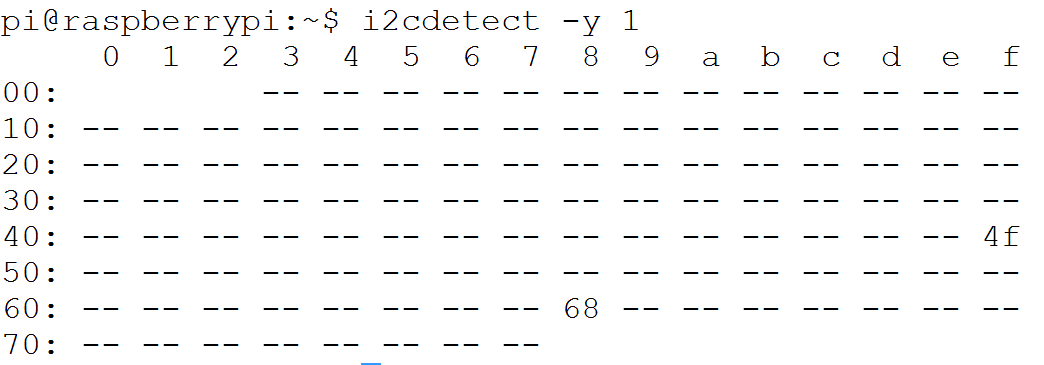
\includegraphics[width=0.5\textwidth]{images/sensorendetect}
	\caption{Hier kann man die zugewiesenen Adressen der Sensoren erkennen: 4f und 68}\label{Fig:imgSensorDetect}
\end{figure}

Konkret besitzt der Car-PC einen GY521 Beschleunnigungssensor und einen DS1621 Temperatursensor. Diese beiden sind für insgesamt etwa 15€ (Stand 04 2016 [amazonquelle]) Online erhältlich.

\begin{figure}[!htb]\centering
   \begin{minipage}{0.49\textwidth}
     \frame{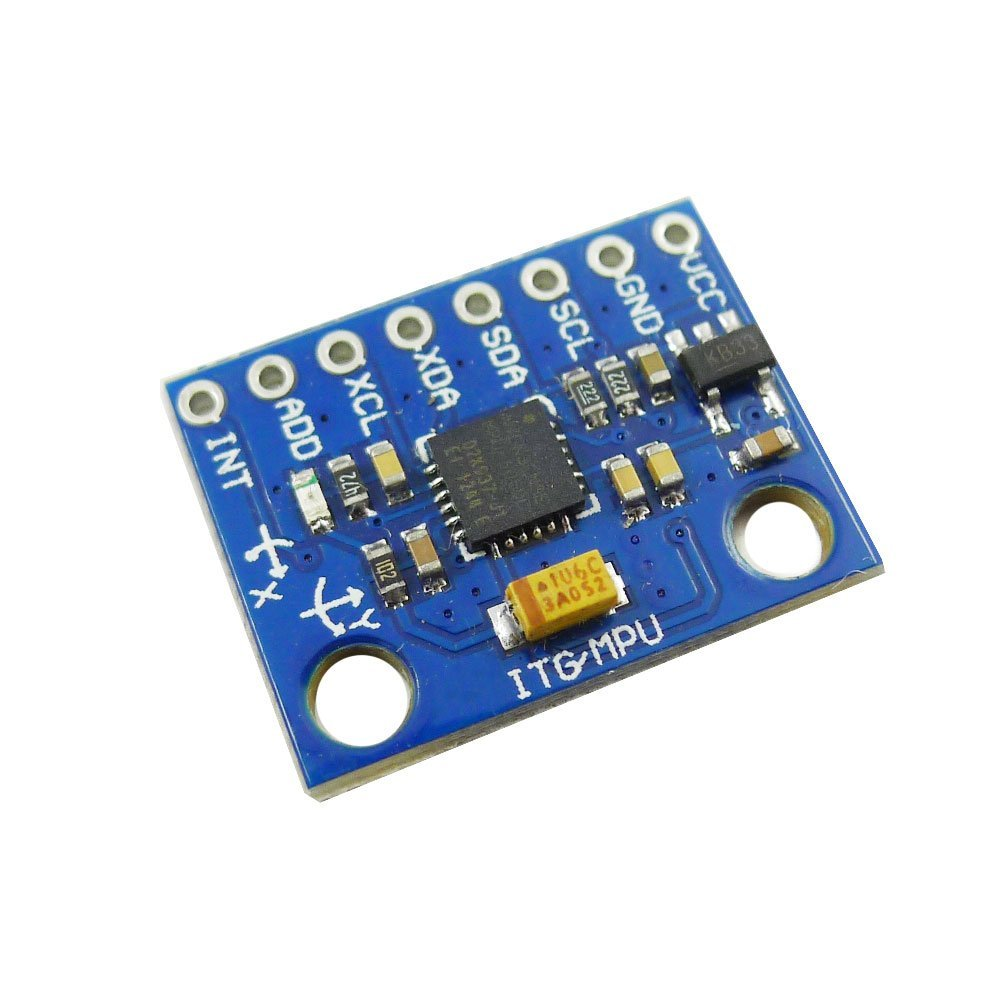
\includegraphics[width=\linewidth]{images/gy521}}
     \caption{Ein GY521 Beschleunigungssensor \cite{PERT.CH3-carpc.gy521}}\label{Fig:imgGY521}
   \end{minipage}
   \begin {minipage}{0.49\textwidth}
     \frame{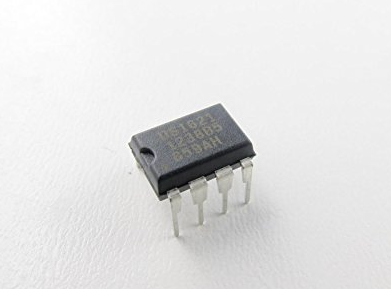
\includegraphics[width=\linewidth]{images/ds1621}}
     \caption{Ein DS1621 Temperatursensor \cite{PERT.CH3-carpc.ds1621}}\label{Fig:imgDS1621}
   \end{minipage}
\end{figure}

Da nicht alle notwendigen Daten direkt aus der OBDII Schnittstelle ausgelesen werden können, wird ein PC gebaut, welcher in die Mittelkonsole eines KFZ integriert werden kann.
Dieser PC soll einen Single-Board PC und Sensoren enthalten, welche eben diese Daten über eine Bluetooth Verbindung an ein Smartphone senden kann.


\clearpage % DO NOT REMOVE